\chapter{Study Evaluation}
\label{chapter:study_evaluation}
\section{Study Evaluation}
\label{sec:study_evaluation}
The study presented in the last chapter is evaluated with the help of a pre pilot study and a pilot study. The pre pilot study was conducted with one person and focused on flaws in the process. Subsequent a pilot study was performed with three participants. The pilot study focus lies on the review of the \exgo and the assessment of data. This section describes the findings of the pilot studies and provides improvements for the actual study.

\subsection{Process}
In the beginning, the participant gets a welcome letter. Regarding the welcome letter, two participant stated that the information about how VR head sets work is not necessary. The welcome letter is shortned by the removal of that passage. The infromed consent is signed. The subsequent demographic questionaire, allows to put the study's data into context. During the review of the produced study data, no further questions occurred. The demographic questionaire needs no further improvements. During the participant reads the welcome letter, the system is set up. The pilot study showed that the time to set up the system and filling the questionaires are corresponding.\\
Afterwards, he participant is told, that he/she will be attached with the trackers and where the trackers will be attached. The trackers are attached to the participant. To respect the privacy of the participant, the trackers are handed to the participant and instructions are given how to attach them. The pilot study showed that the participants had problems to follow the instructions correctly. For the actual study, the participants will be asked if it is ok that the trackers are attached with physical help of the study conductor.\\
Next, the participants received information about what to expect in the VR. The instructions contained information about the GV ("You will see one/multiple teachers.") and the task ("Please follow the instructions of the teachers as exact as possible."). Furthermore, the participant was asked to pay attention to the ergonomics of the movements. Explataions about the speed-mechanic was provided, too ("The teacher will wait for you if you are too far away from the teacher. If thats is happening, correct the placements of your feet and it will go on."). No participant had difficulties to understand the instructions. Additionally, the participant was handed the box, to get used to it before the participant will see it's digital pendant in VR. Finally, the calibration of the system was explained ("Please look into the mirror you will see there (study conductor pointing) and extend your arms like this (study conductor performing the T-pose)"). All participants understood how to calibrate at ease. The introduction of the mirror as calibration help proved to be helpful and suitable.\\
Subsequently, the camera recordings where started the participant performed the first task. In this phase of the study, two error occured which need adjustments to the process. In one case, the wrong task was chosen which made participant 1 (PT1) to perform task 1 (T1) two times in different perspectives. PT1 recognised that, too. Before starting the task, an "is everything ok" checklist should be gone through. The second error regards the identification and synchronisation of the video recordings. At the ceiling a GoPro films the scene from above. A second camara catches the scene from the side of the tracking volume. For identification, a sing was hold into the view of the bot cameras. This was forgotten twice. As improvement I suggest, to place the sign beforehand in the area both camears cover.\\
After the participant performed the first task, the participant took of the HMD and is asked to fill in the after session questionaire. The trackers stayed at the body of the participants. The pilot study showed, that the tracker do not hinder the participants to sit down and fill in the questionaires. In the pilot study, a 3 minute pause was planed to allow the participant to recover. During that pause, the participant was asked for his/hers wellbeeing, to check for VR induced motion sickness. All participants stated that they do not need a pause. Nevertheless, the pause will be maintained, because all participants are expirienced with virtual reality. A person with no prior exposition to VR could feel different.\\
Session two and three are cunducted in the same way as session one. With all three sessions done, the trackers are removed and the semi-structured interview was conducted. Becuase the pilot participants were not payed, the pilot study ended here. The planed duration of the study was 75 minutes. All pilot studies took no longer that 55 minutes.  With an additional buffer, the planed study duration can be decreased by 10 minutes to 65 minutes.\\
Additionally, for evaluation of the study, the participants were interviewd to get insights about the studies and systems flaws. The participants were asked if the explanations were sufficient, things that confused them, unclear questions in the questionaires and the documents. Finally, the participants opinion oabout possible improvements of \exgo and the study were asked. The results of that interviews informed the section~\ref{sec:studyStructure}, too.
To conclude, wide parts of the planed study process proved to be suitable. Adjustments, are made to the welcome letter, the attachment of the trackers with the help of the study conductor, an addidional checklist to check the sessions task and perspective is introduced and the camera recording identification is improved by placing the sign into the recording area beforehand.

\subsection{\exgo}
All hardware artifacts of \exgo are suitable without objections. The study participants rated the box's size and weight as ok while still perceiving the box as "physical load". The tables size is sufficient for all three task. During no task the participants were in danger to collide with a physical artefact. The size of the scale is also sufficient, the box was always placed on the scale safely. The positions and itinerary between mirror, table and scale are without complaint. Regarding the hardware part of \exgo the pilot study revealed two insights, one related to the trackers and one related to the HMD. The tracker at the hip is attached with a strap around the hip of the participant. During the movemennts lift and lower, the tracker is shifted upwards. The upwards shift affects the presentation of the avatar, and unfluences the accuracy measurements hip distance and the RM squat distance, and upright stance. To prevent this, the student was asekd to wear a belt. The tracker belt was then fixated to the participant belt with a band of velcro. This includes touching the participants in the lower hip area from behind. To prevent that participants do not feel uncomfortable during the whole study, the fixation of the two belts should be performed with a clip which can be attached by the participant itself. The second insight regarding the hardware of \exgo is the cable of the HMD. During the study, the study conductor handled the cable to not influence the participant. In one case, the cable was pulged out during a session. \exgo is designed fo that case and plugging in tha cable again allows to continue with the session. However, in the actual study this incident would lead to unusable data for all three session of tha participant, because in the meantime the cable is pluged in again, the GV will move forward and the error will be high during this phase. The acutal study will benefit from a wireless HMD.\\
One participant stated, that he/she could not identify the ownership of the box right away. As soons as the own box is in the hands of the participant it is no problem to tell which is the GV's box and which is the learners box. However, if both boxes a stationary, the participant could not detect which is the own box. For a better destiction between the learner's box and the GV's box, the box should be change to a light transparancy. This will also have an influence of the perception of the box during lift. During lift, the learners box is occluded by the GV's box for a short time. For conformity, the avatar, table and scale of the GV's should also be rendered with a light tanspacrency.\\
The pilot study served as the last test before the actual study. An important part of the pilot study is the review of the produced data. During the development, the measures could only be tested individually. The pilot study allowed for the first time to get a whole image. Fortnuately, most of the logged data worked as intendet, only minor error were detected. For spine bend, a last minute edit caused an incorrect calculation. For EXO in combination with task 2, an invisible error were detected: the props animation controller, wich animates the GV's box, played the wrong task for the ego-centric GV. In EXO, the ego-centric GV is invisible but used to calculate the measurements. For EGO, the learners avatar identification name (used for looking at, to identify on what the learer is cisually focusing) is incorrect. Lastly, Unity3D natively uses comma as decimal seperator. Most statistics programms natively use points as decimal seperator. A log file of one session contains arround 2.5 Million decimal seperators. Converting a log file is time consuming, and thereof, the logging should be changed to use point as decimal seperator.

das zeug aus den questionaires
\subsection{Questionaires}
fragen in den fragebögen müssnen angepasst und erweitert werden.\\

aufgrund der Pilotstudie beschreiben, welche elemente gut bzw schlecht sind.\\

gibt es schwierigkeiten etwas zu verstehen\\

pausen zwischen den sessions\\
sind die anweisungen die gegeben wurden zu viel/zu wenig\\
refinements\\
...\\

\subsection{Acclimatisation Phase}
The first session of each study is the acclimatisation phase, where the learner get used to \exgo. It is assumed, that the learning effect between session one and two is high, and between two and three nearly no learning effect occurs. To evaluate if this assumption holds, the task completion time (TCT) could give insights, because of the speed-mechanic. The speed mechanic regulates the animation speed of the GV based on the distance between learner and GV, and is applied in all perspectives. The higher the distance learner-GV distance, the lower the speed. A learner which is located  often near to the ideal point yields a lower TCT. A formative test in which one participant does all three tasks in the same condition would lead to insights about the learning effect. Such a test was not possible because of the COVID-19 pandemic. Nevertheless, comparing the TCT in the pilot test could at least indicate if the learning effect between session two and three is low by showing similar TCT.\\
Figure~\ref{fig:tct} shows the amount of ms the participants needed more to complete the task compared with the task norm duration (over task norm duration (OTND)). The task norm time is the amount of ms the task needs to complete without the speed-mechanic. The order of the sessions is from left to right. Participant 1 (PT1) had a nearly equal OTND for all three tasks. Because of a mistake in choosing the task during the pilot study, PT1 faced task one two times. Even though, in session three the OTNT is slightly higher.PT2 shows the expected behaviour, having a high OTND in the first session and a nearly equal OTND for session two and three. PT3's OTND is strictly monotonically decreasing. If the OTNT behaviour of all the participants would be like PT2's behaviour, the choice of the acclimatisation method is correct. If the OTNT behaviour for all participants would look like PT3, the acclimatisation method would be incorrect. In this case a seperate condtition specific acclimatisation before every session should be conducted. Unfortunately, the data is ambiguous and does not allow an evaluation of the acclimatisation method. Thereby, using the first session for acclimatisation is maintained.


\begin{figure}[htb]
	\centering
	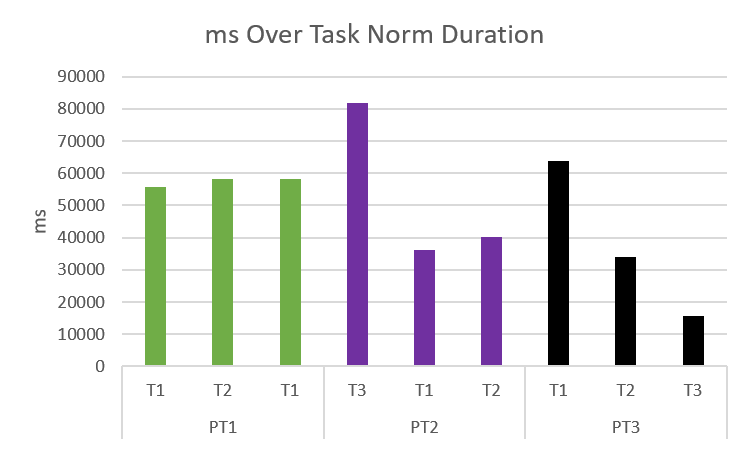
\includegraphics[width=0.8\textwidth]{figures/msOverTaskNorm.png}
	\caption[TCT of all sessions.]{Amount of miliseconds over task norm time (task duration without speed mechanic). PT - participant, T - task.}
	\label{fig:tct}
\end{figure}

\section{Data Analysis}
Based on the pilot study, this section tries to give a first glimps on the data. The data relies on only three participants. Additionally, the data relies on a pilot study. A pilot study serves to identify issues and faults in the system and study and prepare the final study conduction. Section\todo{55} describes found issues and faults and the solution for them. Some issues and fault had an impact on the data, which leaded to the exclusion of corresponding data. Furthermore, as described in section~\ref{sec:studyStructure}, a full counterbalancing of tasks and conditions are possible with nine participants. Additionally, the data revealed in some aspects a high variation in both qualitative and quantitative data. Thereof, the depicted data is a rough estimation and conclusions can not be drawn. The analysis is superficial and a detailed analysis like significats verification is renounced. However, a first impression about a possible outcome can be given. All charts depicted in this section are similar structured. The conditions in all charts have the same colour coding: \textcolor{blue}{EGO} is depicted in blue, \textcolor{orange}{EXO} is depicted in orange and the combination \textcolor{gray}{EGO \& EXO} is depicted in gray. For all charts (except for head angle) hold: the lower the bar, the better in the corresponding context.\\
Firgure~\ref{fig:cumulatedError} can be perceived as an abstract for this section by showing the overall error in distance and angle between the learner and the GV per VP. Overall, the ego-centric VP mostly outperformed both the exo-centric VP and the ego \& exo-centric VP, while the ego \& exo-centric VP mostly socred better than the exo-centric VP.
\begin{figure}[htb]
	\centering
	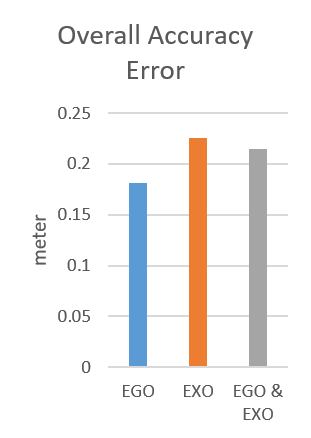
\includegraphics[width=0.3\textwidth]{figures/cumulatedDistanceError.png}
	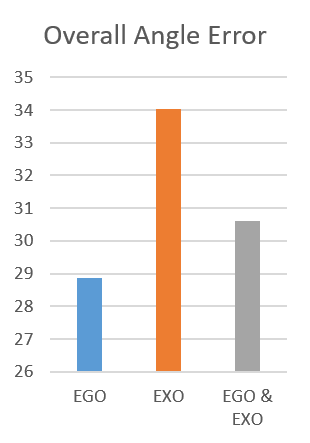
\includegraphics[width=0.3\textwidth]{figures/cumulatedAngleError.png}
	\caption[Cumulated error per perspective.]{Cumulated average distance error (left) and angle error (right) per VP.}
	\label{fig:cumulatedError}
\end{figure}


\subsection{Accuracy}
Accuracy is clustered by distance and angle, and applied for the body parts hands, feet, hip, head and box. Distance is the Euclidean distance between the learners e.g. hand and the GV hand in meters and describes the difference in position. Angle describeds the difference in orientation and is measured in degrees. The overall error per body is depicted in~\ref{fig:overallError}.
Section~\ref{sec:studyStructure} showed that some subtasks can be aggregated into pairs, based on the smililarity of the movements: lift/lower, push/pull, turn/fold and pick/place. Figure~\ref{fig:avgErrorPerSubTask} shows the average error in distance and angle per sub-task and confirms the pairing of the sub-tasks by showing a realation between the pairs. Hence, in the following, the pairs of sub-tasks will be analysed in combination. Carry, walk are analysed standalone. This section is structured by the sub-tasks. The sub-task is analyised based on the accuracy measurements and compared with the subjective accuracy of the learner.
\begin{figure}[H]
	\centering
	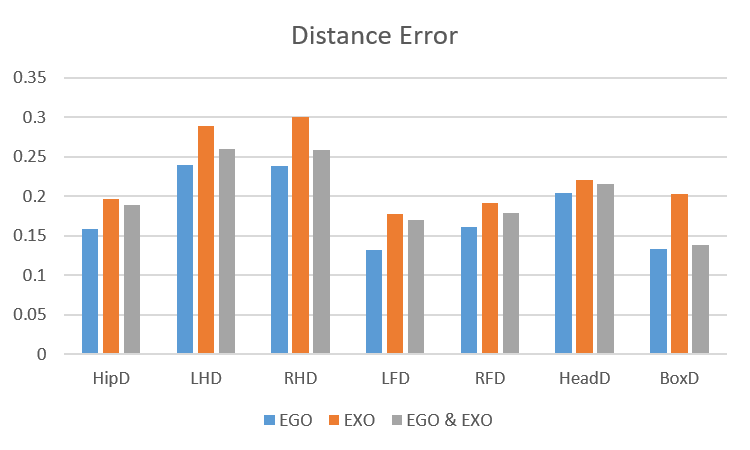
\includegraphics[width=0.49\textwidth]{figures/overallDistanceError.png}
	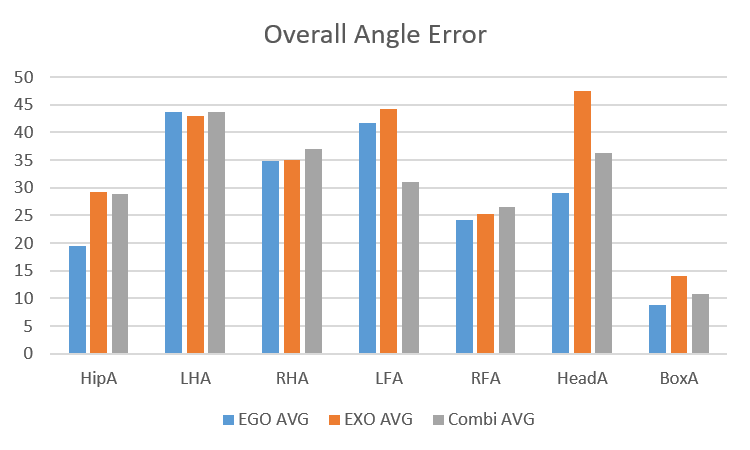
\includegraphics[width=0.49\textwidth]{figures/overallAngleError.png}
	\caption[Average error per body part in meter.]{Average error per body part. Left: distance error, right: angle error. Suffix D: distance, suffix A: angle. LH - left hand, RH - right hand, LF - left foot, RF - right foot.}
	\label{fig:overallError}
\end{figure}
\begin{figure}[H]
	\centering
	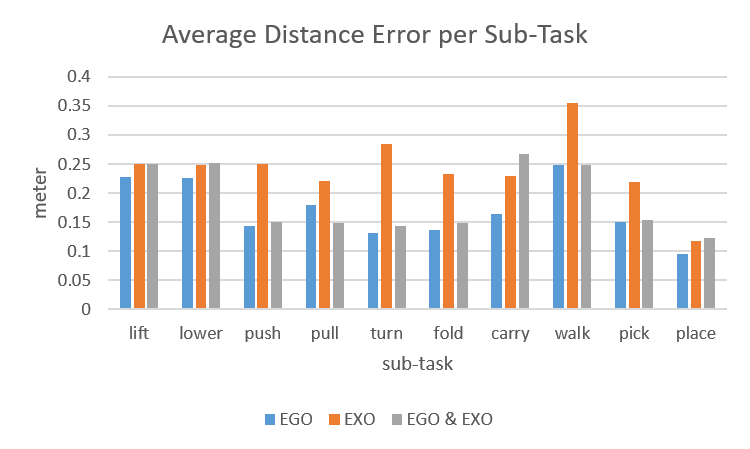
\includegraphics[width=0.49\textwidth]{figures/averageDistanceErrorPerSubTask.png}
	\includegraphics[width=0.49\textwidth]{figures/averageAngleErrorPerSubTask.png}
	\caption[Average error of sub-task\textit{carry}]{Average error of sub-task \textit{carry}. Left: distance error, right: angle error. Suffix D: distance, suffix A: angle. LH - left hand, RH - right hand, LF - left foot, RF - right foot.}
	\label{fig:avgErrorPerSubTask}
\end{figure}
	
Figure~\ref{fig:overallError} shows that the distance error of hands and the error of feet are related. This is expected since large parts have synchronised movements, for example, the hands touch the box simultaneously. Across all conditions, the feet's error is lower than the hand's error. The hand's error is lower in EGO than in EXO. Hands are directly visible in front of the learner and the direct comparison to the ego-centric GV is a possible explanation. Suprisingly, feet's error is lower in EGO, too. To see the feet, the learner must actively move the head, especially if the box blocks the view on the feet. However, it seems easier to aling the learners feet with the GV feet in EGO. The box distance and angle error is lower in EGO and \combi. The presence of an ego-centric GV box increases the distance and angle accuracy for the box persumable significatntly. The hip error indicates to what exctend the learner could determine the correct location. The data indicates that the determination of the own position and rotation is easier with an ego-centric GV. The head angle is not comparable with the other accuracy measures. The presence multiple of exo-centric GVs in the EXO forces the learner to look into different directions. The difference between EXO and \combi could point out, that the learner focused in \combi on both, the exo-centric GVs and ego-centric GV. The angle based accuracy for the hand and feet receal no clear trend. More participants are needed to get a clearer view. Overall, the presence of an ego-centric GV increases the distance accuracy for all body parts. For the box shaped physical load, the presence of an ego-centric GV increases the angle accuracy, too. On the one hand, it seems that adding exo-centric GVs to the ego-centric GV decreases the distance accuracy. A possible reason could be that the learner shares the focus with multiple GV, or that the presece of four exo-centric GVs overwhelms the learner. The study participants rated their overall accuracy highest in EGO and lowest in \combi, compare~\ref{fig:overallSubjectiveAccuracy} (left). The subjective low accuracy in \combi would underpin the theory that the learners where overwhelmd. But when the participants where asked for their subjective accuracy for the body parts arms, legs and back, a different picture araises, compare~\ref{fig:overallSubjectiveAccuracy} (left). The opinion of the participants are differentiated which causes a high standard deviation of around 1.5 on a Likert scale from 1-7. More participants could lead to a clearer view. At the other hand, adding an ego-centric GV to exo-centric GVs increases the accuracy slightly.\\
The described insights rely on the whole task containing all sub-tasks. Though, the drawn deductions are only true for a task that includes all sub-tasks in the same amount. Potentionally, the accuracy in specific sub-tasks could deffer from the overall accuracy. In the following, the sub-tasks are analysed and vetted if the deductions count for the specific sub-tasks.
\begin{figure}[H]
	\centering
	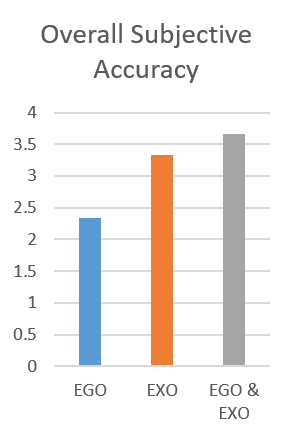
\includegraphics[width=0.3\textwidth]{figures/overallSubjectiveAccuracy.png}\\ 
	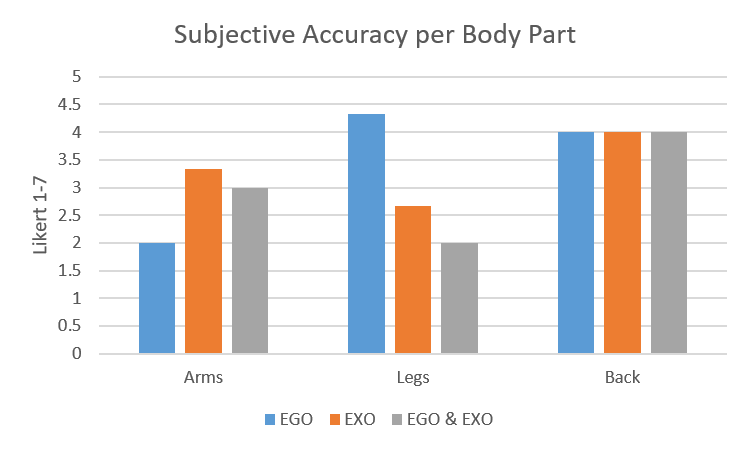
\includegraphics[width=0.49\textwidth]{figures/subjectiveAccuracyPerBodyPart.png}
	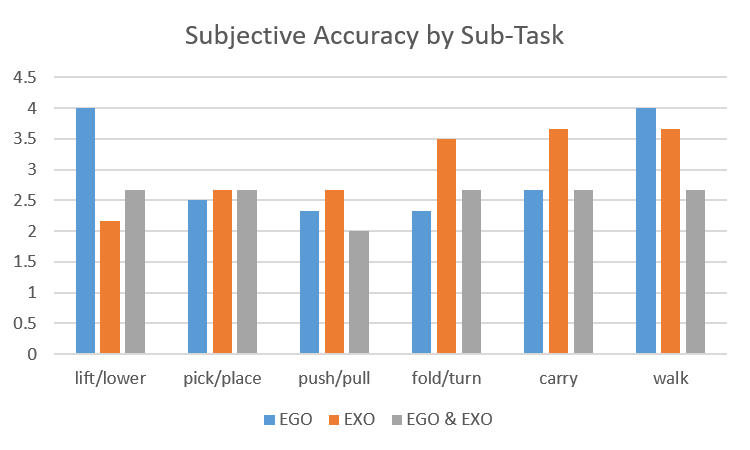
\includegraphics[width=0.49\textwidth]{figures/subjectiveAccuracyBySubTask.png}
	\caption[Subjective accuracy per VP]{Subjective accuracy per VP}
	\label{fig:overallSubjectiveAccuracy}
\end{figure}

\begin{figure}[H]
	\centering
	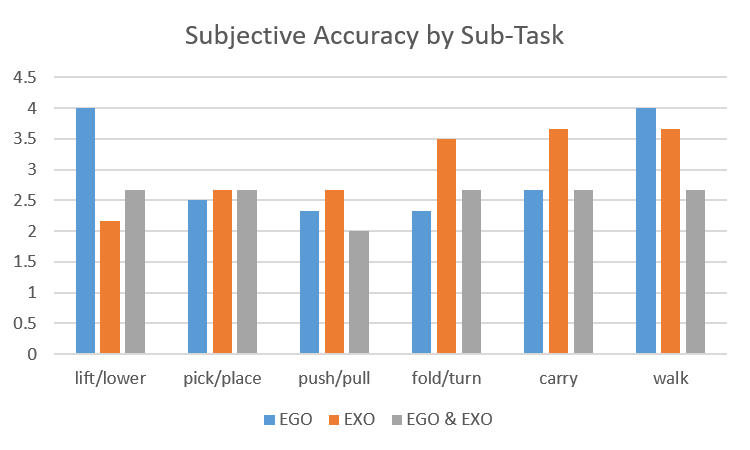
\includegraphics[width=0.29\textwidth]{figures/subjectiveAccuracyBySubTask.png}
	\caption[Subjective accuracy per sub-task]{Subjective accuracy per sub-task}
	\label{fig:subjectiveAccuracybySubTask}
\end{figure}

\subsection{lift/lower}
\begin{figure}[H]
	\centering
	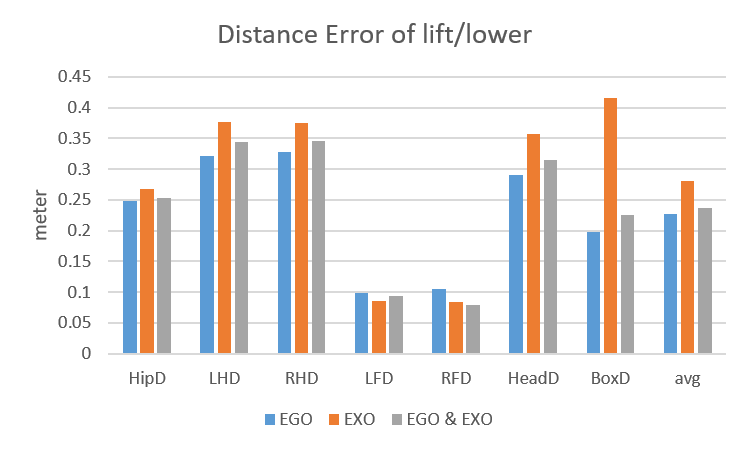
\includegraphics[width=0.49\textwidth]{figures/distanceErrorLiftLower.png}
	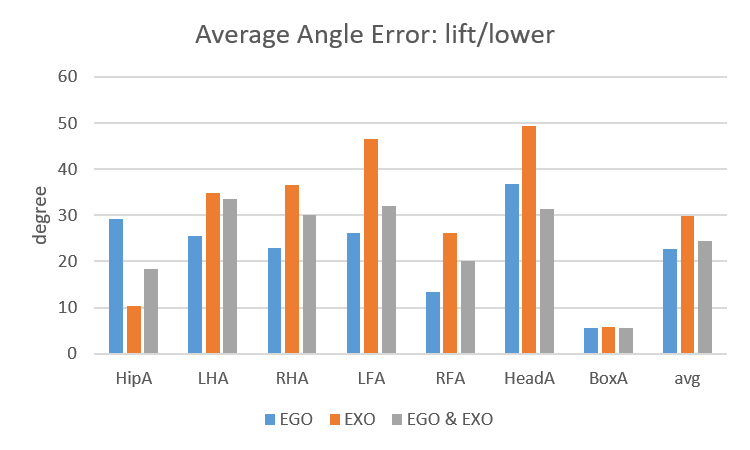
\includegraphics[width=0.49\textwidth]{figures/angleErrorLiftLower.png}
	\caption[Average error per body part for sub-tasks lift/lower.]{Average error per body part for sub-tasks lift/lower. Left: distance error, right: angle error. Suffix D: distance, suffix A: angle. LH - left hand, RH - right hand, LF - left foot, RF - right foot.}
	\label{fig:errorLiftLower}
\end{figure}
Figure~\ref{fig:errorLiftLower} shows that in EGO the hip, hand and head accuracy is higher than in an EXO. The presence of exo-centric GV seem to have a positive influence on the feet accuracy. The box's accuracy in EXO is lower than in EGO and EXO. In the actual study, special attention shuold be paid to the box during lift and lower to identify the cause why EXO performes bad. In orientation, the box's error is low for all VPs. This is expected, since the sub-task does not include a change in orientation.
The subjective accuracy is by far lowest in EGO, followed by EGO and EXO.

\subsection{pick/place}
\begin{figure}[H]
	\centering
	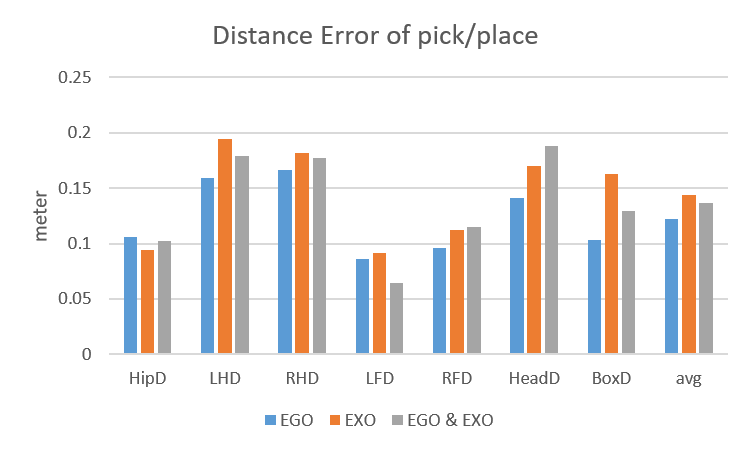
\includegraphics[width=0.49\textwidth]{figures/distanceErrorPickPlace.png}
	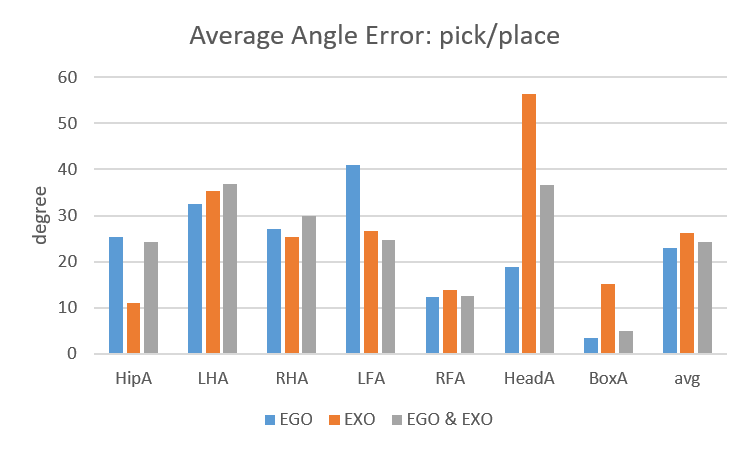
\includegraphics[width=0.49\textwidth]{figures/angleErrorPickPlace.png}
	\caption[Average error per body part for sub-task turn/fold.]{Average error per body part for sub-task turn/fold. Left: distance error, right: angle error. Suffix D: distance, suffix A: angle. LH - left hand, RH - right hand, LF - left foot, RF - right foot.}
	\label{fig:errorPickPlace}
\end{figure}
Pick and place are lift and lower movements with a significant difference in magnitude. The accuracy of pick and place benefits from the presence of an ego-centric GV. The distance and angle error of the box is lowest in EGO.
\subsection{push/pull}
\begin{figure}[H]
	\centering
	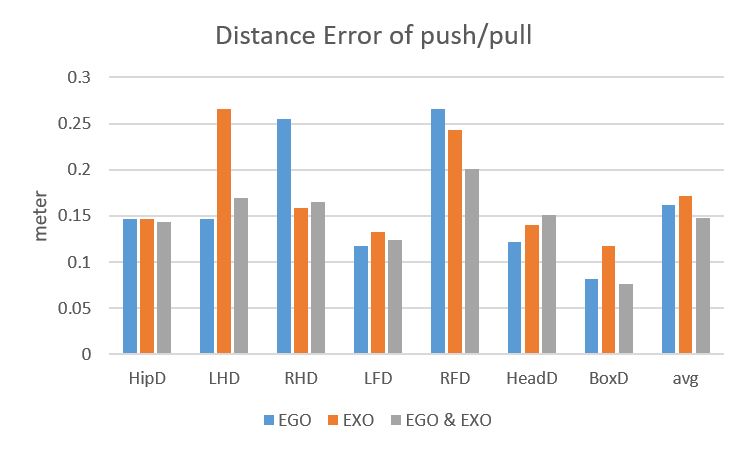
\includegraphics[width=0.49\textwidth]{figures/distanceErrorPushPull.png}
	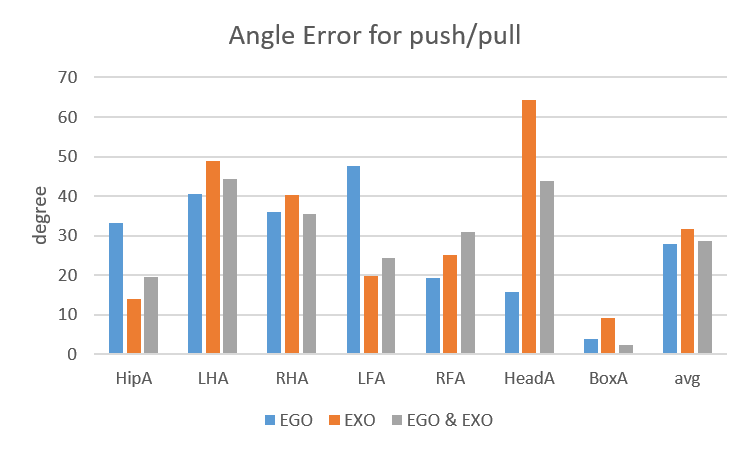
\includegraphics[width=0.49\textwidth]{figures/angleErrorPushPull.png}
	\caption[Average error per body part for sub-tasks push/pull.]{Average error per body part for sub-tasks push/pull. Left: distance error, right: angle error. Suffix D: distance, suffix A: angle. LH - left hand, RH - right hand, LF - left foot, RF - right foot.}
	\label{fig:errorPushPull}
\end{figure}
During push and pull, increased force is applied to the box. Because of the increased force application, the physiologist suggested that for push and pull, one foot should be schifted to the back. The high difference in error between the left foot and right foot is based on different foot placement. Unfortunately, the participants realised the different foot placement in no condition. In the interview, one participant stated that he did not realise to shift one foot back in EGO. But in EXO he saw it and applied it then also for \combi. This statement harmonises with the quantitative data, which shows the lowest accuracy in EGO. The left hand seems to have a high error in EXO, the right hand in EGO. The video revealed that the participants alternated the hand placement during push and pull. Based on the video observation, the high error could even out with more participants. The higher error of the head angle in EXO compared to \combi indicates that the participants shared the focus in \combi with the ego-centric GV and the exo-centric GV. The participants rated their movements more exact in \combi than in EGO, and lowest in EXO.

\subsection{turn/fold}
\begin{figure}[H]
	\centering
	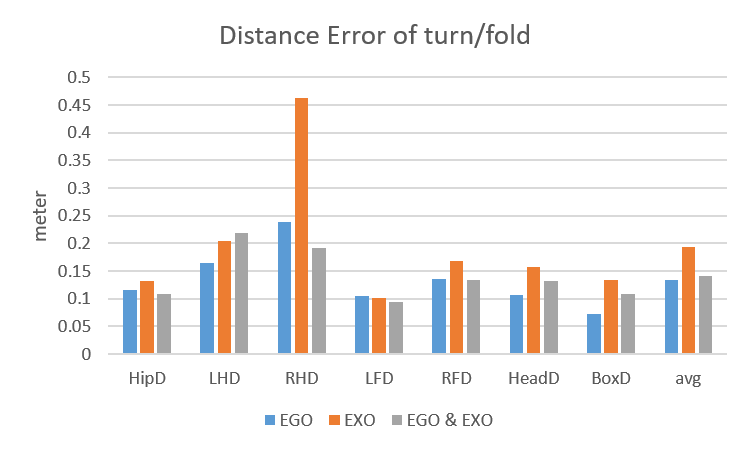
\includegraphics[width=0.49\textwidth]{figures/distanceErrorTurnFold.png}
	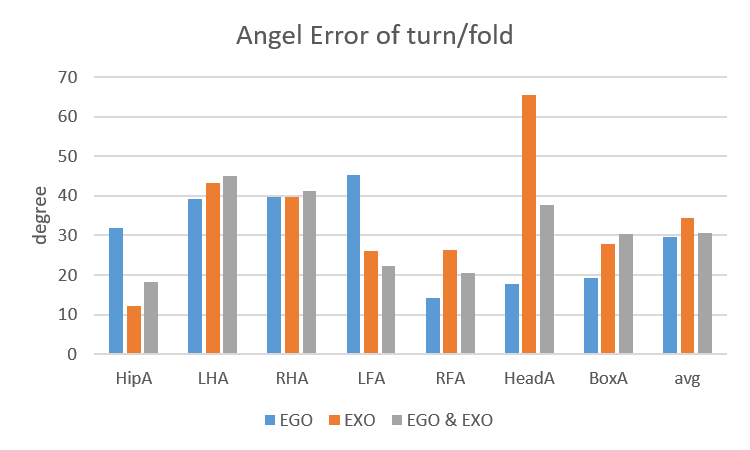
\includegraphics[width=0.49\textwidth]{figures/angleErrorTurnFold.png}
	\caption[Average error per body part for sub-task turn/fold.]{Average error per body part for sub-task turn/fold. Left: distance error, right: angle error. Suffix D: distance, suffix A: angle. LH - left hand, RH - right hand, LF - left foot, RF - right foot.}
	\label{fig:errorTurnFold}
\end{figure}
The most of the movements during turn and fold happen on the table, thus the main focus is on the hands. The high error in EXO is noticable. The consultation of the video recordings revealed that in EXO, the participants could not see directly the direction of turn and changed the right hand after the movement began. Furthermore, after starting to turn or fold the box, the participants changed the position of the hand, persumably to ease the movement. The perceived accuracy is highest in EGO, followed by \combi and EXO. 

\subsection{carry and walk}
\begin{figure}[htb]
	\centering
	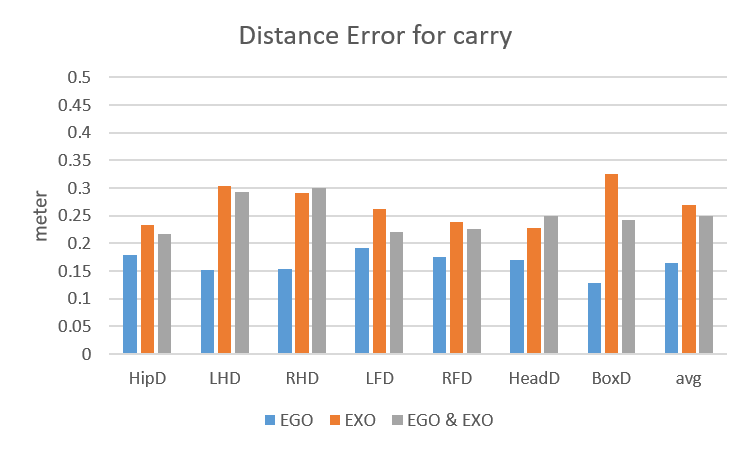
\includegraphics[width=0.49\textwidth]{figures/distanceErrorCarry.png}
	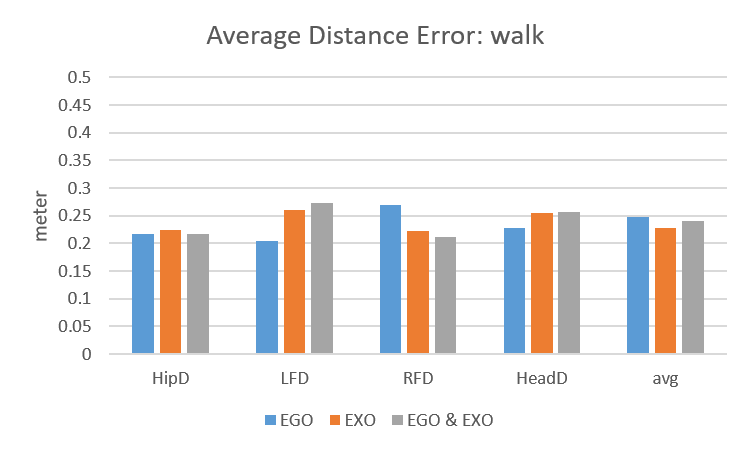
\includegraphics[width=0.49\textwidth]{figures/distanceErrorWalk.png}
	\caption[Average error of sub-tasks \textit{carry} and \textit{walk}]{Average error of sub-tasks  \textit{carry} (left) and \textit{walk} (right). Suffix D: distance. LH - left hand, RH - right hand, LF - left foot, RF - right foot.}
	\label{fig:walkError}
\end{figure}
Teaching locomotion in the ego-centric VP with the help of the speed-mechanic is a novetly. The data revealed an nearly equal error for ego-centric guided walking and exo-centric guided walking. The position of the hands are not important for walking and are not depicted. Adding a phyical load to walking (carry), has a strong influence on the accuracy. The learner seems to focus on the box and tries to match the GV's box with the own box. This increases the accuracy of the own position for all body parts.

\section{Visual Focus}
In EGO, the learner is provided one ego-centric GV and will focus on it. If exo-centric GV are added to the scene, the learner can focus on multiple GVs. Furthermore, it is interesting which percentage of time the learner focuses on the own/GVs box and own/GVs body.\\
\begin{figure}[htb]
	\centering
	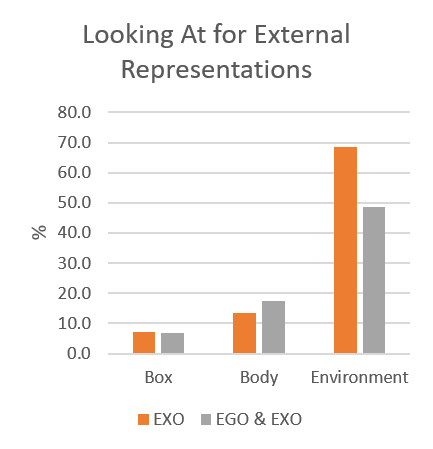
\includegraphics[width=0.5\textwidth]{figures/lookingAtExternalRepresentations.png}
	\caption[Looking At for external representations.]{When looking on an external representation, percentage of time focusing on the box or table.}
	\label{fig:lookingAtExternal}
\end{figure}
A pilot study helps to evaluate the experiment design and the data aquisition. Conducting a pilot study before the actual study is vital. The proove is depicted in figure~\ref{fig:lookingAtExternal}. In section~\ref{sec:rayTrace} is described how the looking at data aquisition method was developed and tested. The formative test was conducted with one person\footnote{More participants were not possible because of the COVID-19 pandemic.}, which is too less. The study data revealed that the data aquistion for looing at is not working correctly. Over 50\% of time the ray traces hit the environment. For the actual study, the colliders of the artefacts and avatars should be adjusted, or if available, an eye-tracker should be used. Nevertheless, assuming the rays which hit something else than the enivronment are evently distributed, some deductions can be made from the aquired data.\\
Figure~\ref{fig:lookingAtExternal} shows the percentage of time, the learner focused on the a box, a body (avatar) and the enviornment. The learner foccused roughly twice as much on a body than on the box.\\
Figure~\ref{fig:posHeatMap} shows the positions of the GVs whereby a GV is the union of body, table and box. The positions are overlayed with a heat map. The orange circles stand for the percentage of time the learner focussed on that position. The heat map provides two insights. First, the presence of an ego-centric GV influences the visual focus of the learner. In EXO, where no ego-centric GV is present, the learner focused 11\% of the time on the own table and box. In \combi, the learner focused 45\% of the time on the ego-centric GV. If an ego-centic GV is present it is more fequently focused than exo-centric GVs. By implication, the learner is consulting the exo-centric GVs, if an ego-centric GV is present.
The second insight regards position four. In EXO and \combi, the learner did not focus on the GV at position four. Position four is superfluous for all three tasks.
\begin{figure}[htb]
	\centering
	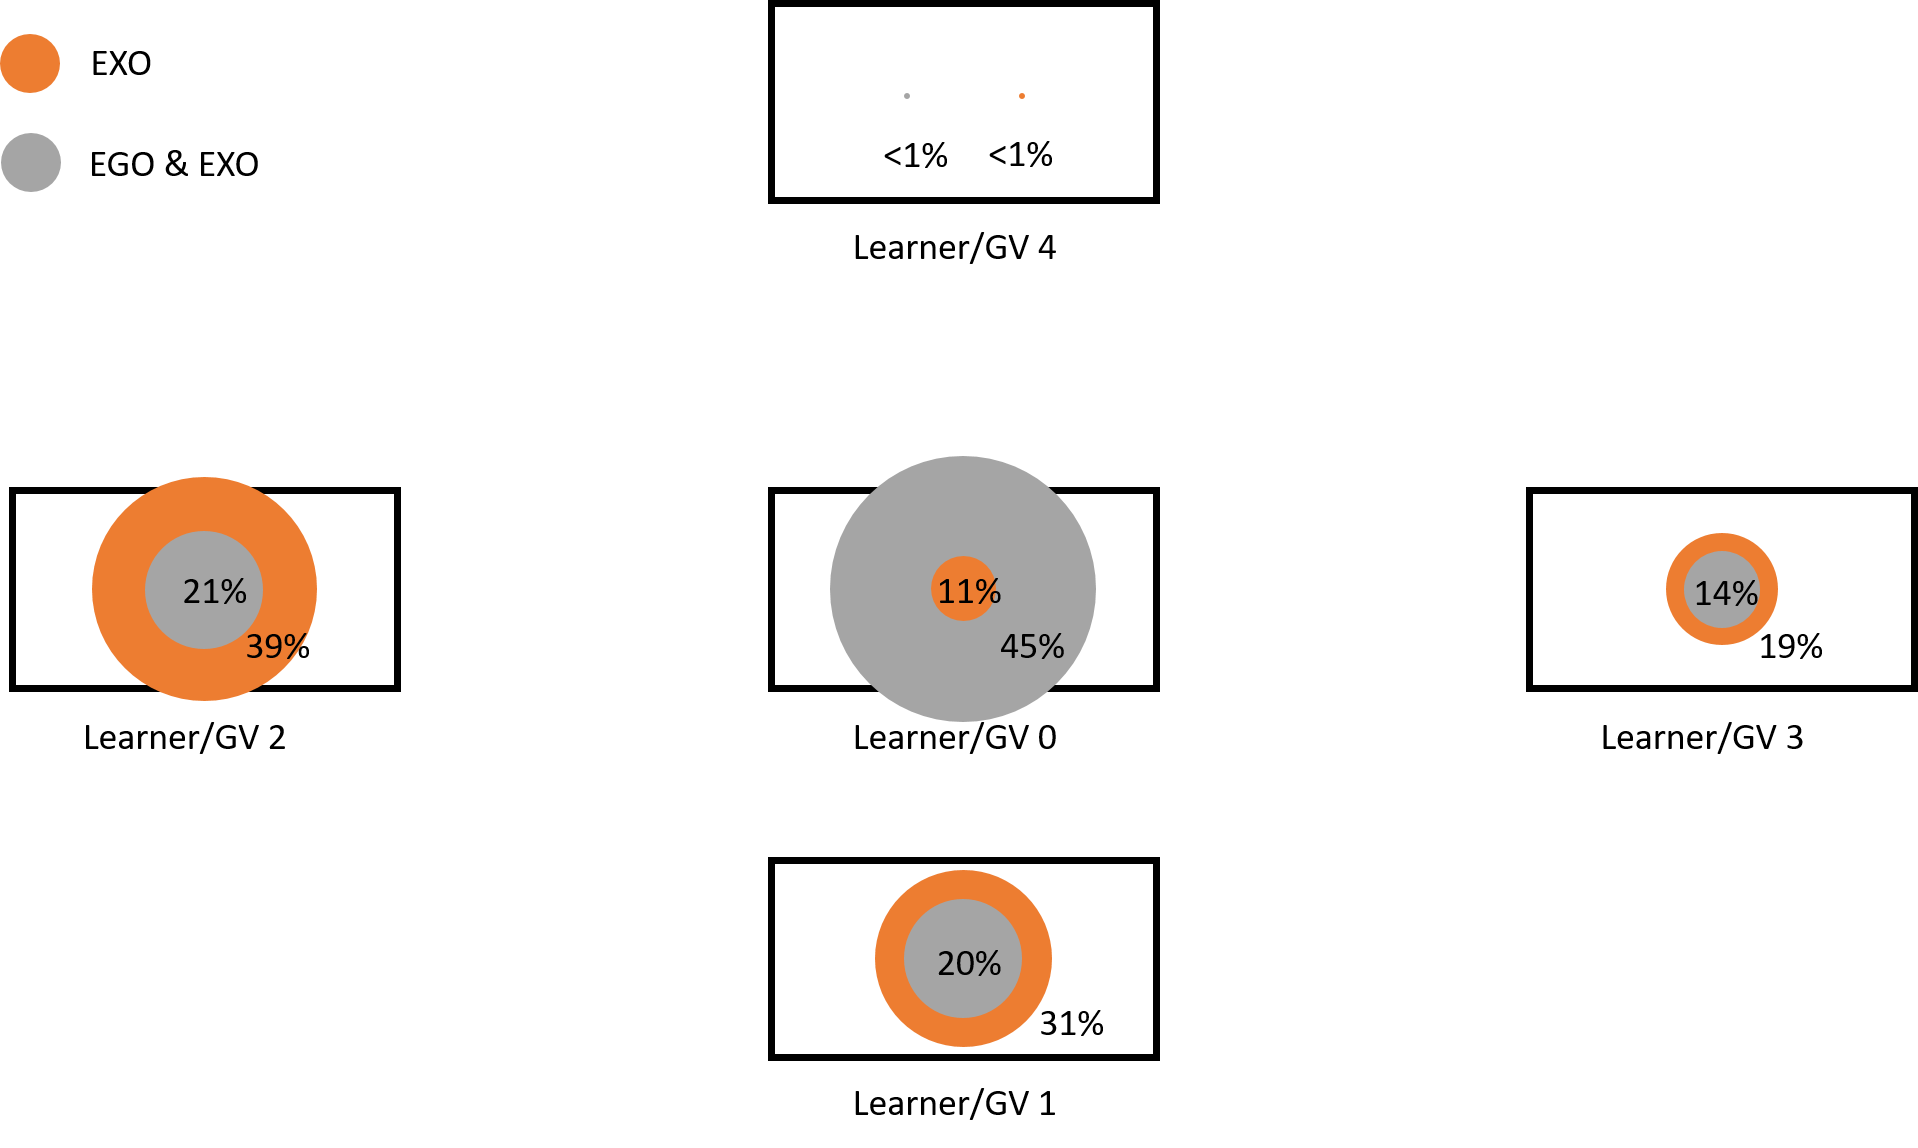
\includegraphics[width=\textwidth]{figures/positionHeatMap.png}
	\caption[Looking At heat map.]{Heat map of the learners focus in EXO and EGO \& EXO. The heatmap shows the tables of the multiple representations. The circles's size correspond to the amount of time the leaner focused the representation.}
	\label{fig:posHeatMap}
\end{figure}
percieved acc per body part

\section{Risk Measurements}
The Risk Measurements are not analysed. The reason refers to the missing windows the Risk Measurements are based on. Recap: for specific sub-tasks the specific Risk Measurement should be between a minimum and a maximum. The time inside and outside the window between minimum and maximum yield a score. To determine a window fo the Risk Measurements, best a professional is consulted. Because of the COVID-19 pandemic a determination by a professional was not possible.\\
However, the accuracy data for lift and lower could lead to a guess to the performance of squat distance. The feet accuracy is higher in EXO than in EXO. Squat distance refers to the same body part. Thereby, the assumption seems legit, that squat distance could be better in perspectives with an exo-centric GV. Good Base and Spine Bend are refering to body parts that are not directly visible in EGO, though, the assumption could be extended to Good Base and Spine Bend, too.

\section{Subjective Preferences}
The personal preferences of the participants tend towards perspectives with exo-centric GVs. If the participants had the choice of choosing a VP for the task, two would decide for \combi and one would use EXO. Additionally, two participants stated, that they could follow the GV best in \combi, one could folow the GV best in EGO. All but one participants ranked the ability to follow the GV worst in EGO. This competes with the accuracy which is lowest in EGO. Suprisingly, all participants stated that the easiest VP was EGO. In EGO the GV stands inside the own body, which is not possible in real-world scenarios. Limitation for the ease of understanding is the high proficiency and knowlesge about VR of all participants.
